\documentclass[12pt,a4paper]{article}

% Basic packages
\usepackage[T1]{fontenc}
\usepackage{geometry}
\usepackage{graphicx}
\usepackage{amsmath}
\usepackage{algorithm}
\usepackage{algorithmic}
\usepackage{enumitem}
\usepackage{abstract}
\usepackage{booktabs}
\usepackage{microtype}
\usepackage{float}
\usepackage{titlesec}
\usepackage[acronym]{glossaries}
\makeglossaries

% Typography and spacing
\usepackage{setspace}
\onehalfspacing

% Page layout
\geometry{
    margin=1in,
    headheight=14.5pt
}

% Font configuration
\usepackage{fontspec}
\setmainfont{Arial}
\newglossaryentry{hedera}{
    name={Hedera},
    description={A public distributed ledger technology that uses a hashgraph consensus algorithm}
}


% Captions and figures
\usepackage{caption}
\usepackage{subcaption}
\captionsetup{
    format=hang,
    labelfont=bf,
    textfont=it
}

% Tables
\usepackage{tabularx}
\usepackage{booktabs}

% Headers and footers
\usepackage{fancyhdr}
\pagestyle{fancy}
\fancyhf{}
\fancyhead[R]{\thepage}
\fancyhead[L]{AutoTrust - Vehicle Lifecycle Platform}
\renewcommand{\headrulewidth}{0.4pt}

% Hyperlinks (must be loaded last)
\usepackage{hyperref}
\hypersetup{
    colorlinks=true,
    linkcolor=blue,
    filecolor=magenta,
    urlcolor=cyan,
    pdftitle={AutoTrust - Vehicle Lifecycle Platform},
    pdfauthor={Muzaffar Ahmed, Dharmendra Agrawal},
    pdfsubject={Vehicle Management System on Hedera Network},
    pdfkeywords={blockchain, vehicle management, hedera, smart contracts}
}

% Cross-referencing (must be loaded after hyperref)
\usepackage{cleveref}
\crefname{figure}{Figure}{Figures}
\crefname{table}{Table}{Tables}
\crefname{section}{Section}{Sections}

% Code listings
\usepackage{minted}
\usemintedstyle{vs}
\setminted{
    frame=lines,
    framesep=2mm,
    baselinestretch=1.2,
    fontsize=\footnotesize,
    linenos
}

% List spacing configuration
\setlist[itemize,1]{itemsep=0.5em,parsep=0.5em}
\setlist[enumerate,1]{itemsep=0.5em,parsep=0.5em}
\setlist[itemize,2]{itemsep=0.25em,parsep=0.25em}
\setlist[enumerate,2]{itemsep=0.25em,parsep=0.25em}

% Title formatting
\titleformat{\section}
{\normalfont\Large\bfseries}
{\thesection}
{1em}
{}
\titleformat{\subsection}
{\normalfont\large\bfseries}
{\thesubsection}
{1em}
{}

\begin{document}

    \begin{titlepage}
        \centering
        
\includegraphics[width=0.3\textwidth]{CSE-IITM-Logo.png}\par
        \vspace{1cm}
        {\Large\textbf{Indian Institute of Technology--Madras (IIT--Madras)}\par}
        \vspace{0.5cm}
        {\large\textbf{Department of Computer Science and Engineering}\par}
        \vspace{0.5cm}
        {\large\textbf{M.Tech in Computer Science \& Engineering}\par}
        \vspace{1cm}
        {\Large\textbf{CS6858: Distributed Trust}\par}
        \vspace{1cm}
        {\Huge\bfseries AutoTrust - Vehicle Lifecycle Platform\par}
        \vspace{2cm}
        {\Large\textbf{Instructor:}}\par
        {\large Prof. John Augustine}\par
        \vspace{0.5cm}
        {\Large\textbf{Teaching Assistant:}}\par
        {\large Barath Ashok}\par
        \vspace{1cm}
        {\Large\textbf{Students:}}\par
        {\large Muzaffar Ahmed (CS23M517)}\par
        {\large Dharmendra Agrawal (CS23M508)}\par
        \vspace{2cm}
        {\large April 18, 2025\par}
    \end{titlepage}

    \clearpage
    \pagenumbering{roman}
    \setcounter{tocdepth}{2}
    \tableofcontents
    \clearpage
    \pagenumbering{arabic}


    \section{Project Summary}
    This project implements a decentralized Vehicle Management System on the \gls{hedera} Network, leveraging blockchain technology for secure and transparent vehicle registration and management. The system provides a tamper-proof solution for vehicle registration, ownership transfer, and user profile management. By utilizing smart contracts and distributed ledger technology, it ensures data integrity and transparency while eliminating the need for centralized authority.


    \section{Acknowledgements}
    We would like to express our gratitude to:
    \begin{itemize}
        \item Prof. John Augustine (CSE Dept., IIT Madras) for his guidance and inspiring work in distributed trust and secure distributed computing
        \item Barath Ashok (MS Scholar, IIT Madras) for his teaching assistance
        \item The Hedera development team for their documentation and tools
    \end{itemize}


    \section{Problem Statement}
    The vehicle reselling market suffers from several challenges that can be effectively addressed through blockchain technology:

    \begin{itemize}
        \item Centralized authority leading to single points of failure
        \begin{itemize}
            \item Risk of system downtime
            \item Vulnerability to cyber attacks
            \item Dependence on single authority
        \end{itemize}

        \item Lack of transparency in vehicle history
        \begin{itemize}
            \item Difficulty in verifying past ownership
            \item Hidden accident history
        \end{itemize}

        \item Vulnerability to data tampering
        \begin{itemize}
            \item Manual record manipulation
            \item Unauthorized modifications
            \item Lack of audit trail
        \end{itemize}

        \item Inefficient verification processes
        \begin{itemize}
            \item Time-consuming manual checks
            \item Multiple agency coordination
            \item Paper-based documentation
        \end{itemize}

        \item Limited accessibility and interoperability
        \begin{itemize}
            \item Geographic restrictions
            \item System incompatibility
            \item Data silos
        \end{itemize}
    \end{itemize}


    \section{Motivation \& Objectives}

    \subsection{Motivation}
    The motivation behind this project stems from several key factors:

    \begin{itemize}
        \item Need for a transparent and secure vehicle management system
        \begin{itemize}
            \item Growing concerns about vehicle-related fraud
            \item Increasing demand for transparent transactions
            \item Need for reliable vehicle history
        \end{itemize}

        \item Elimination of fraudulent activities in vehicle registration
        \begin{itemize}
            \item Prevention of duplicate registrations
            \item Reduction in stolen vehicle registrations
            \item Elimination of fake documentation
        \end{itemize}

        \item Decentralization of vehicle ownership records
        \begin{itemize}
            \item Distributed storage of records
            \item Elimination of single point of control
            \item Enhanced system resilience
        \end{itemize}

        \item Enhanced trust in vehicle transactions
        \begin{itemize}
            \item Verifiable ownership history
            \item Transparent transaction records
            \item Immutable data storage
        \end{itemize}
    \end{itemize}

    \subsection{Objectives}
    The primary objectives of this project are:

    \begin{itemize}
        \item Develop a decentralized vehicle management system
        \begin{itemize}
            \item Implement blockchain-based architecture
            \item Design secure smart contracts
            \item Create user-friendly interface
        \end{itemize}

        \item Implement secure smart contracts for vehicle registration
        \begin{itemize}
            \item Design efficient data structures
            \item Implement access control mechanisms
            \item Ensure transaction security
        \end{itemize}

        \item Create a user-friendly interface for system interaction
        \begin{itemize}
            \item Design intuitive UI/UX
            \item Implement responsive design
            \item Ensure cross-platform compatibility
        \end{itemize}

        \item Ensure data integrity through blockchain technology
        \begin{itemize}
            \item Implement cryptographic verification
            \item Maintain audit trails
            \item Ensure data immutability
        \end{itemize}

        \item Enable seamless vehicle ownership transfers
        \begin{itemize}
            \item Streamline transfer process
            \item Automate verification steps
            \item Ensure secure transactions
        \end{itemize}
    \end{itemize}


    \section{System Architecture}
    \begin{figure}
        \centering
        \fbox{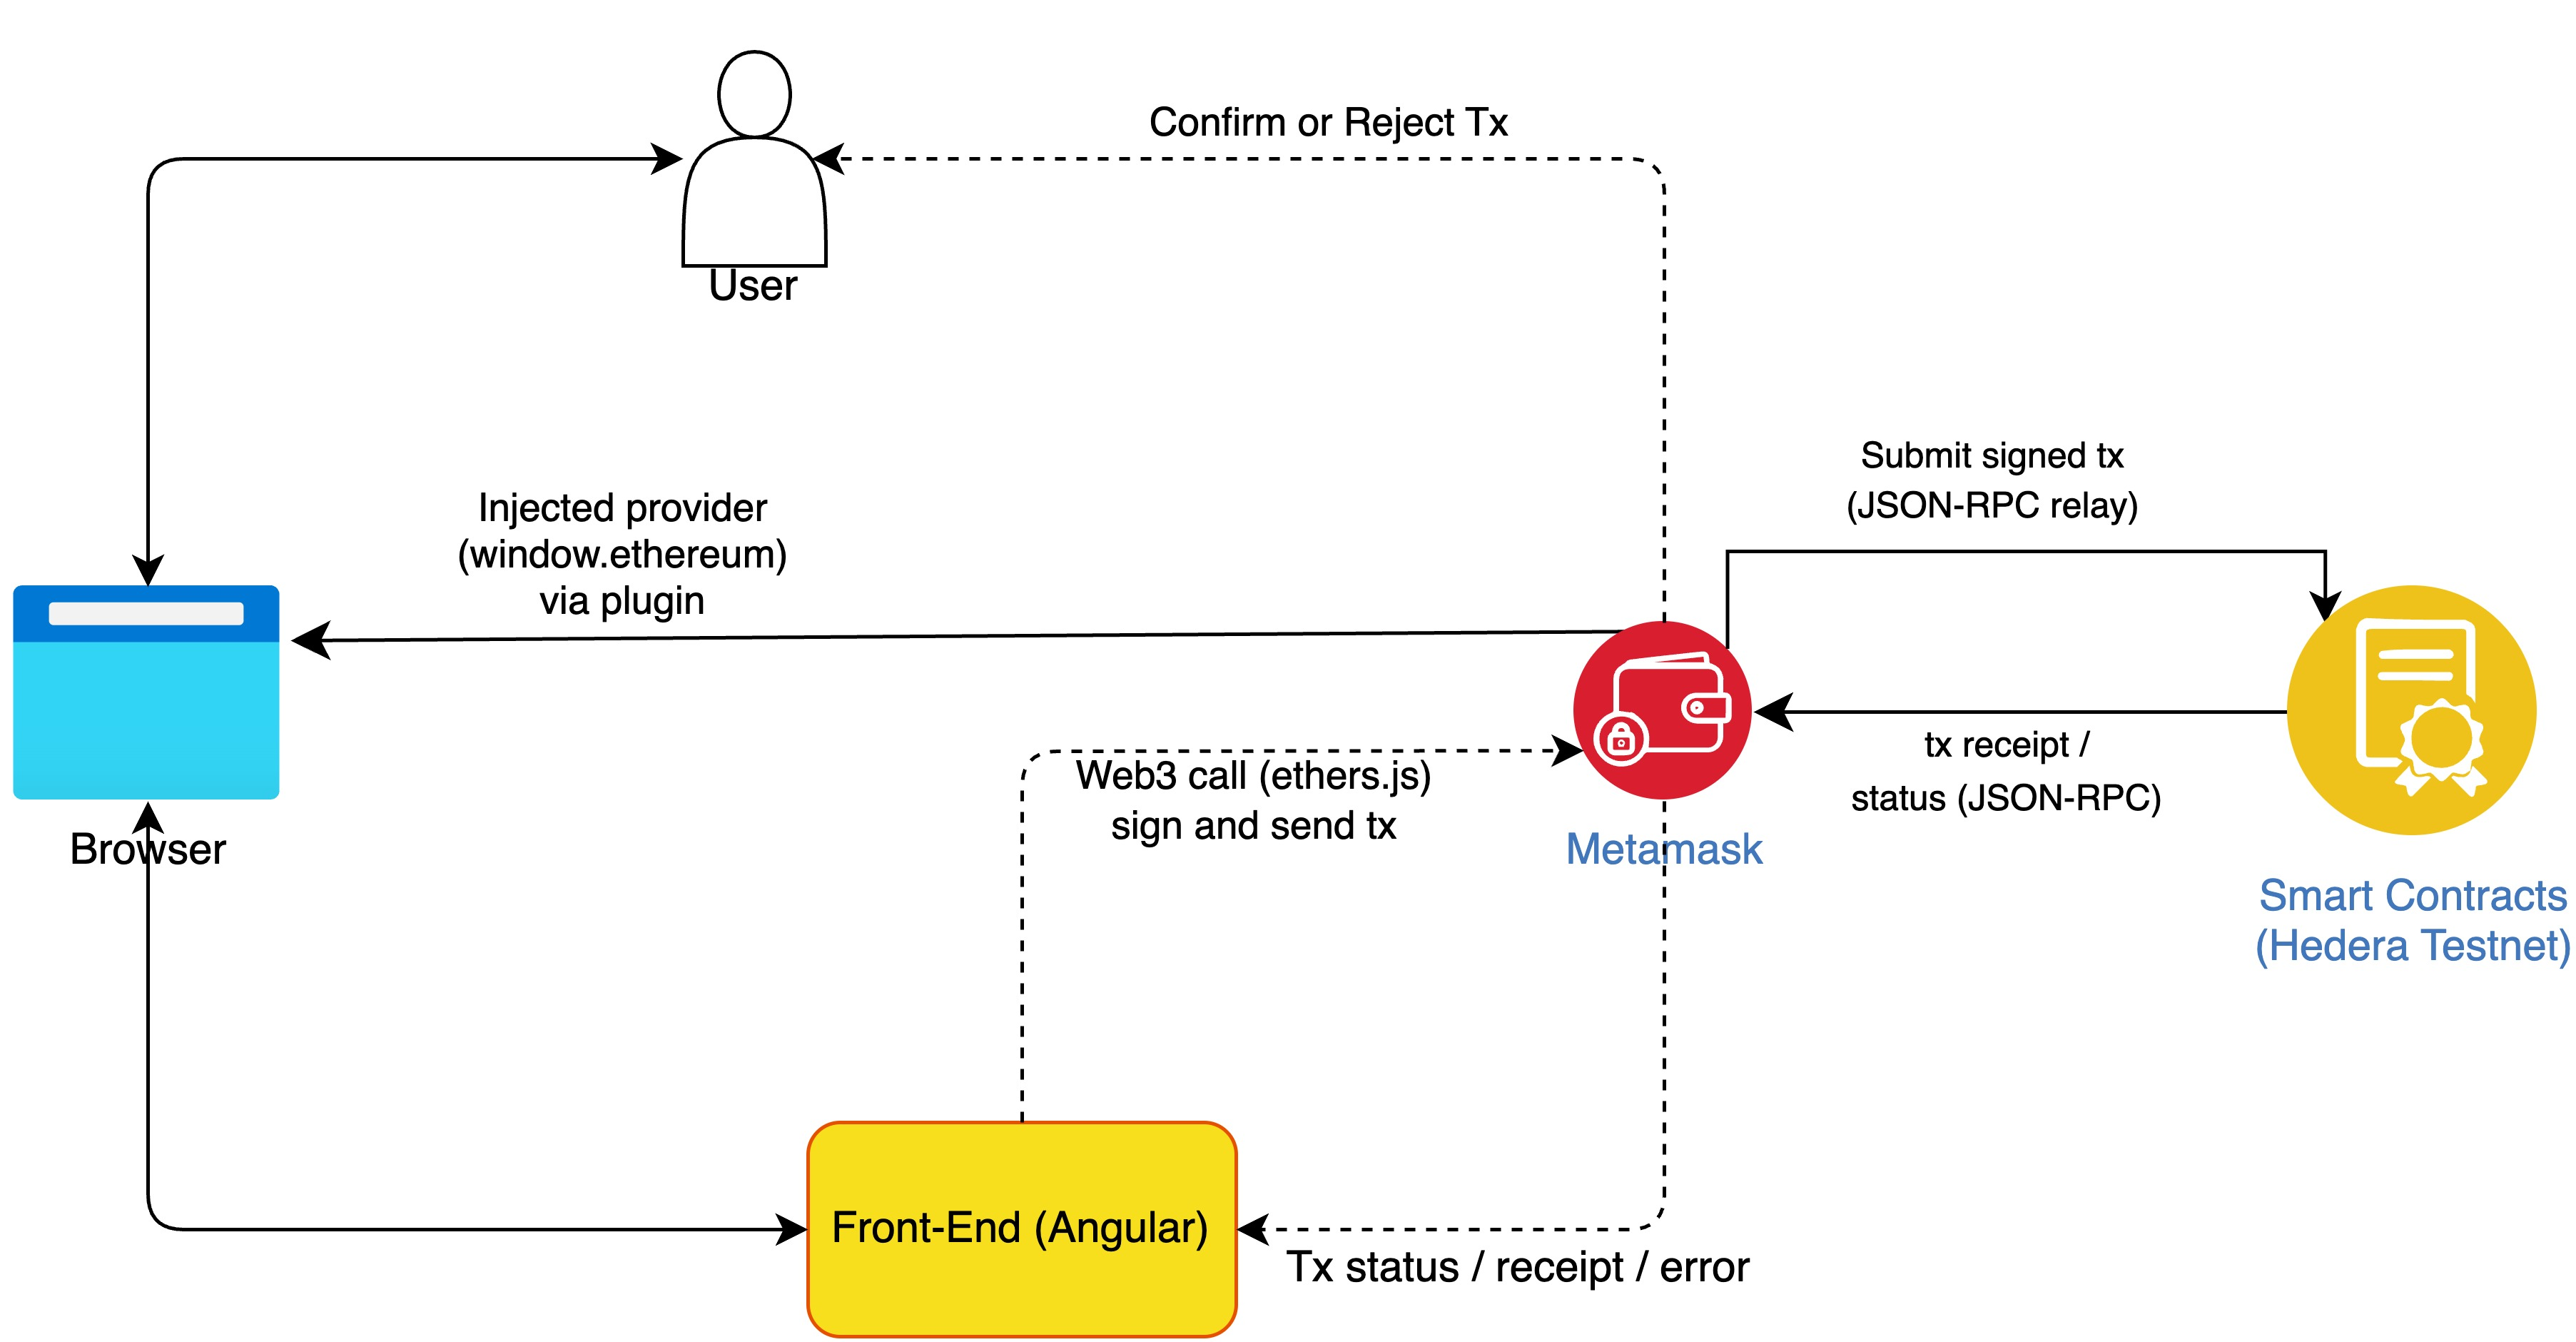
\includegraphics[width=0.8\textwidth]{architecture.jpg}}
        \caption{System Architecture Diagram}
        \label{fig:architecture}
    \end{figure}

    The system follows a decentralized architecture with the following components:

    \subsection{Frontend Layer}
    \begin{itemize}
        \item Angular Application
        \begin{itemize}
            \item User Interface Components
            \item Service Layer
            \item State Management
        \end{itemize}

        \item Web3 Integration
        \begin{itemize}
            \item MetaMask Wallet Connection
            \item Transaction Management
            \item Event Handling
        \end{itemize}
    \end{itemize}

    \subsection{Blockchain Layer}
    \begin{itemize}
        \item Smart Contracts
        \begin{itemize}
            \item VehicleLedger Contract
            \item UserProfile Contract
            \item Access Control
        \end{itemize}

        \item Hedera Network
        \begin{itemize}
            \item Consensus Mechanism
            \item Transaction Processing
            \item State Management
        \end{itemize}
    \end{itemize}

    \subsection{Storage Layer}
    \begin{itemize}
        \item IPFS Storage
        \begin{itemize}
            \item Document Storage
            \item Image Storage
            \item Metadata Management
        \end{itemize}

        \item Local Storage
        \begin{itemize}
            \item User Preferences
            \item Cache Management
            \item Session Data
        \end{itemize}
    \end{itemize}


    \section{Technology Stack}

    \subsection{Frontend}
    \begin{itemize}
        \item Angular
        \begin{itemize}
            \item Component-based Architecture
            \item Reactive Forms
            \item HTTP Client
            \item Router Module
        \end{itemize}

        \item TypeScript
        \begin{itemize}
            \item Type Safety
            \item Object-Oriented Programming
            \item Interface Definitions
        \end{itemize}

        \item SCSS for styling
        \begin{itemize}
            \item Modular Styles
            \item Responsive Design
            \item Theme Support
        \end{itemize}

        \item ethers for blockchain interaction
        \begin{itemize}
            \item Contract Interaction
        \end{itemize}

        \item MetaMask for wallet integration
        \begin{itemize}
            \item Account Management
            \item Transaction Signing
        \end{itemize}
    \end{itemize}

    \subsection{Backend/Smart Contracts}
    \begin{itemize}
        \item Solidity for smart contracts
        \begin{itemize}
            \item Contract Development
            \item Security Best Practices
            \item Gas Optimization
        \end{itemize}

        \item Hedera Network for blockchain
        \begin{itemize}
            \item Consensus Service
            \item Token Service
            \item Smart Contract Service
        \end{itemize}

        \item Node.js for contract deployment
        \begin{itemize}
            \item Contract compilation and deployment Scripts
        \end{itemize}

        \item IPFS for distributed storage
        \begin{itemize}
            \item Document Storage
            \item Distributed application deployment
        \end{itemize}
    \end{itemize}


    \section{Smart Contract Design}
    The system consists of two main smart contracts. For complete code listings, please refer to Appendix \ref{app:contracts}.

    \subsection{VehicleLedger Contract}
    The VehicleLedger contract manages vehicle registration and ownership transfers. Key features include:
    \begin{itemize}
        \item Vehicle registration with owner, registration number and manufacturing year
        \item Ownership transfer with resale amount tracking
        \item Maintenance history management
        \begin{itemize}
            \item Date of maintenance
            \item Type of maintenance
            \item Service provider details
        \end{itemize}
        \item Insurance history tracking
        \begin{itemize}
            \item Insurance reference number
            \item Document hash
            \item Document link
        \end{itemize}
        \item Accident history recording
        \begin{itemize}
            \item Accident date
            \item Report document hash
            \item Report document link
        \end{itemize}
        \item Complete vehicle history retrieval
        \begin{itemize}
            \item Basic details
            \item Past owners
            \item Maintenance records
            \item Insurance records
            \item Accident records
            \item Resale history
        \end{itemize}
    \end{itemize}

    \subsection{UserProfile Contract}
    The UserProfile contract handles user management and authentication. Key features include:
    \begin{itemize}
        \item User profile management
        \begin{itemize}
            \item Name and phone number updates
            \item Vehicle ownership tracking
            \item Automatic profile creation
        \end{itemize}
        \item Vehicle ownership management
        \begin{itemize}
            \item Add vehicles to user profile
            \item Remove vehicles from profile
            \item List all owned vehicles
        \end{itemize}
        \item Profile information retrieval
        \begin{itemize}
            \item Get user details
            \item Get owned vehicles
            \item Get wallet address
        \end{itemize}
    \end{itemize}


    \section{Application Workflow}

    \subsection{User Registration}
    \begin{enumerate}
        \item Connect MetaMask wallet
        \begin{itemize}
            \item Initialize Web3 provider
            \item Request account access
            \item Verify network connection
        \end{itemize}

        \item Create user profile
        \begin{itemize}
            \item Enter name and phone number
            \item Profile automatically created
            \item No additional documents required
        \end{itemize}

        \item Profile verification
        \begin{itemize}
            \item Verify wallet address
            \item Check profile creation
            \item Confirm successful registration
        \end{itemize}
    \end{enumerate}

    \subsection{Vehicle Registration}
    \begin{enumerate}
        \item Submit vehicle details
        \begin{itemize}
            \item Registration number
            \item Year of manufacturing
            \item Verify ownership
        \end{itemize}

        \item Complete registration
        \begin{itemize}
            \item Sign transaction
            \item Pay registration fee
            \item Receive confirmation
        \end{itemize}

        \item Add vehicle history
        \begin{itemize}
            \item Maintenance records
            \item Insurance details
            \item Accident reports
        \end{itemize}
    \end{enumerate}

    \subsection{Vehicle Transfer}
    \begin{enumerate}
        \item Initiate transfer request
        \begin{itemize}
            \item Enter vehicle registration number
            \item Specify new owner address
            \item Set resale amount
        \end{itemize}

        \item Verify ownership
        \begin{itemize}
            \item Check current ownership
            \item Verify transfer rights
            \item Validate transaction
        \end{itemize}

        \item Complete transfer
        \begin{itemize}
            \item Sign transfer agreement
            \item Process transaction
            \item Update ownership records
        \end{itemize}

        \item Update profiles
        \begin{itemize}
            \item Remove from seller's profile
            \item Add to buyer's profile
            \item Record resale amount
        \end{itemize}
    \end{enumerate}


    \section{UI Components}

    \subsection{Core Pages}
    \begin{table}[H]
        \begin{tabular}{@{}p{4cm}p{11cm}@{}}
            \toprule
            \textbf{Page}        & \textbf{Key Features}                                                                    \\
            \midrule
            Login \& Home Page   & Connect wallet; overview; quick actions; navigation tabs                                 \\
            Vehicle Page         & View and update maintenance, accident, past owners and insurance details; resale vehicle \\
            Vehicle Registration & New vehicle registration                                                                 \\
            Search Vehicle       & Advanced filters; results display                                                        \\
            Search User          & Lookup by address; results preview                                                       \\
            User Profile         & Personal info; document management; activity history                                     \\
            \bottomrule
        \end{tabular}
        \caption{Core UI Pages and Features}
        \label{tab:ui-pages}
    \end{table}

    \subsection{Login \& Home Page}
    \begin{itemize}
        \item Ask user to connect MetaMask wallet
        \item Dashboard overview, quick actions, navigation tabs
    \end{itemize}
    \begin{figure}[H]
        \centering
        \subfloat[Request to connect Wallet]{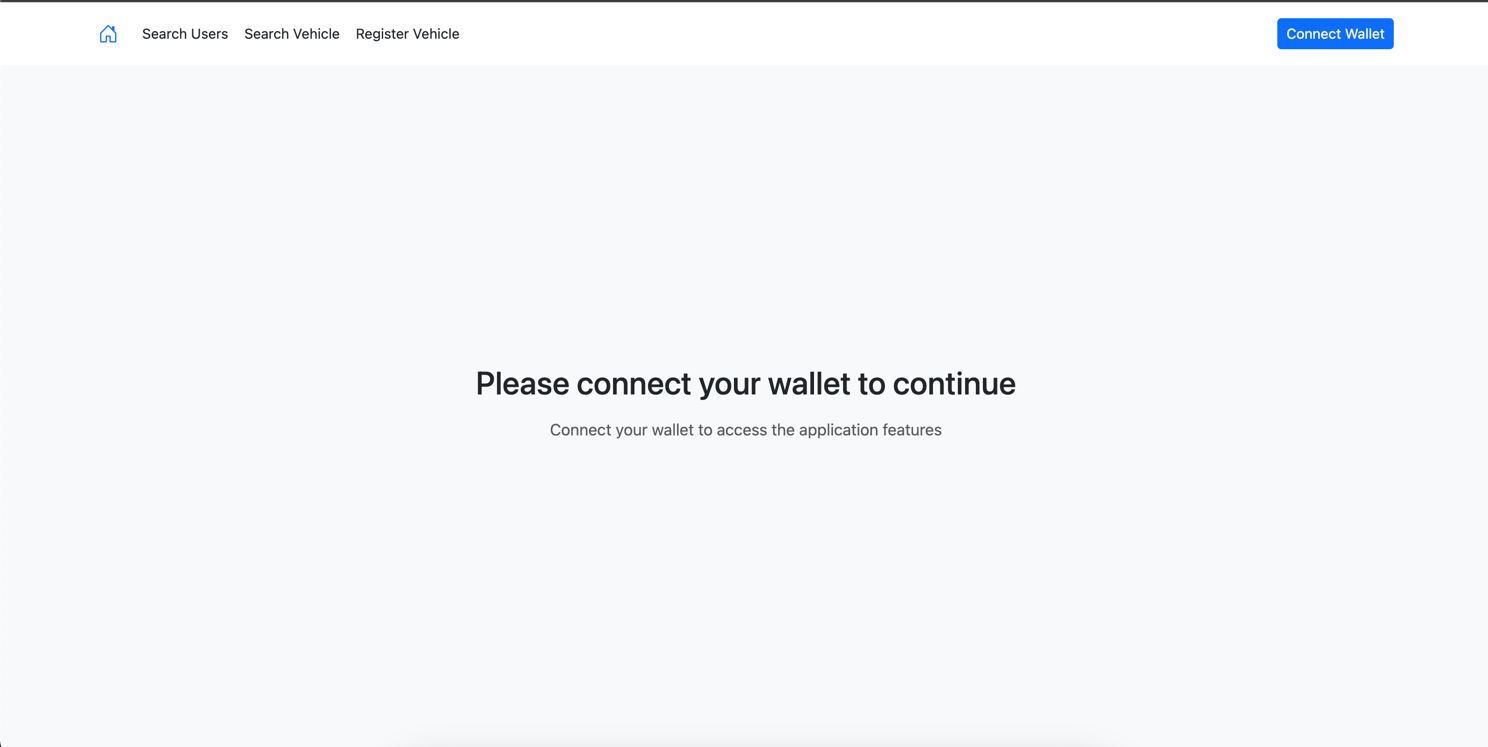
\includegraphics[width=0.45\textwidth]{screenshots/request to connect wallet.png}}\quad
        \subfloat[Home Page]{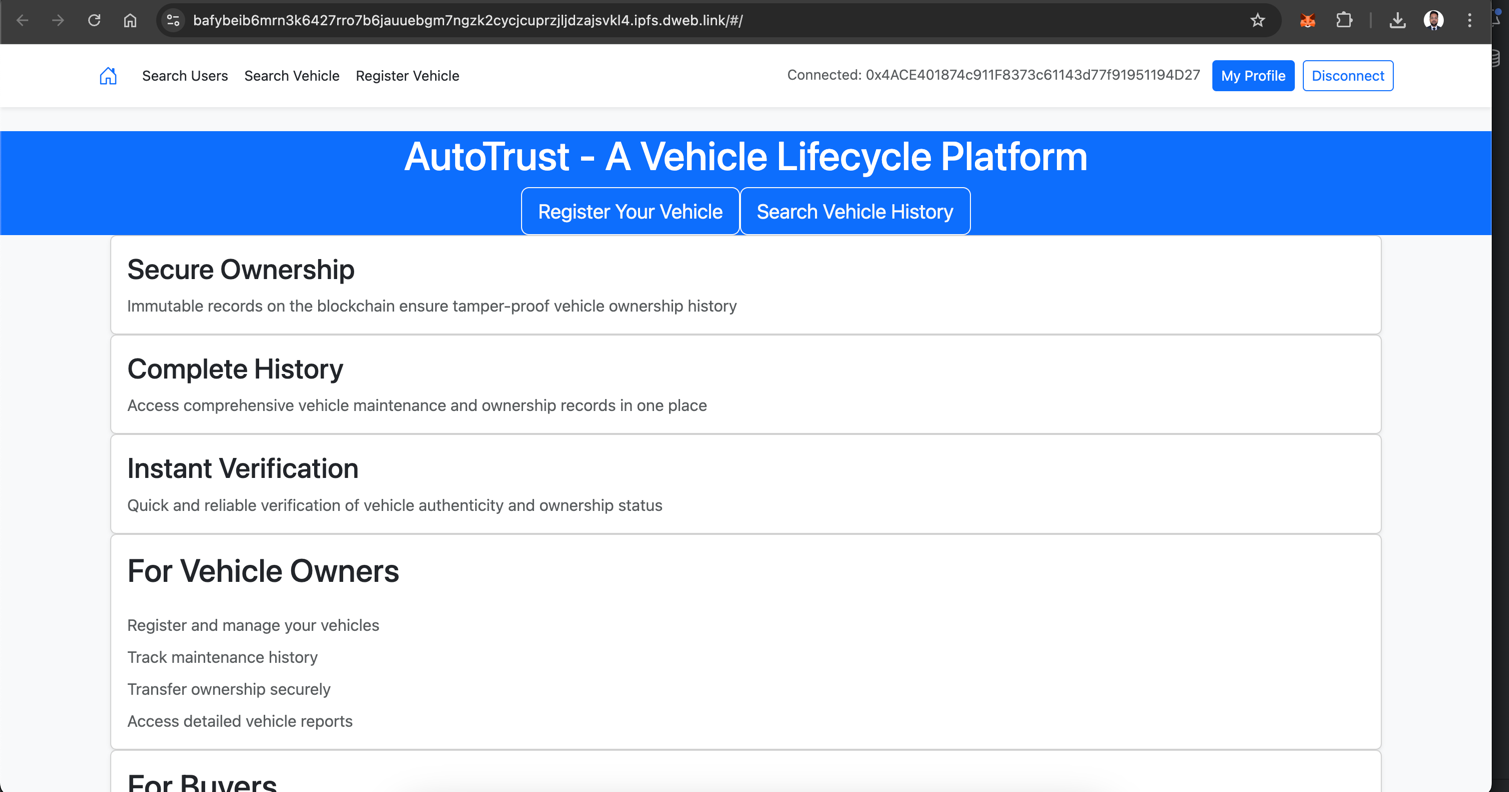
\includegraphics[width=0.45\textwidth]{screenshots/home page after connecting to metamask.png}}
        \caption{Login and Home Page}
        \label{fig:login-home}
    \end{figure}

    \subsection{Vehicle Registration}
    \begin{figure}[H]
        \centering
        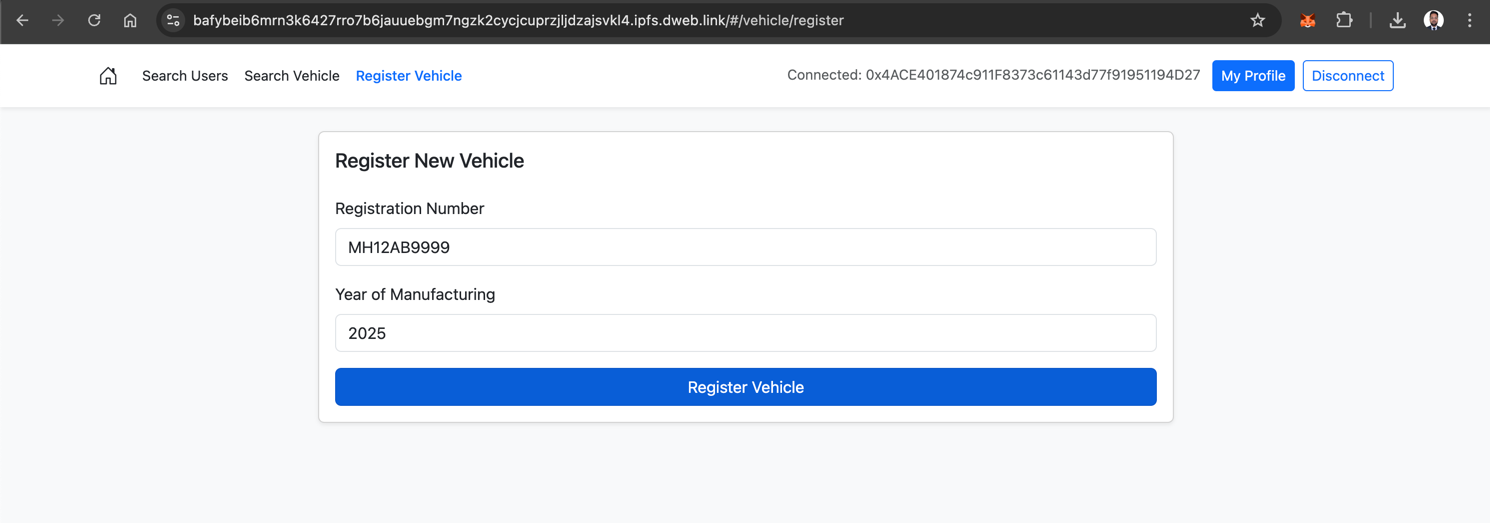
\includegraphics[width=0.6\textwidth]{screenshots/register vehicle.png}
        \caption{Vehicle Registration Form}
        \label{fig:registration}
    \end{figure}

    \subsection{Vehicle Page}
    \begin{itemize}
        \item View basic details
        \item View history: maintenance, accident, past owners, insurance
        \item Buttons to update details and resell vehicle
    \end{itemize}
    \begin{figure}[H]
        \centering
        \subfloat[Basic Details \& Maintenance]{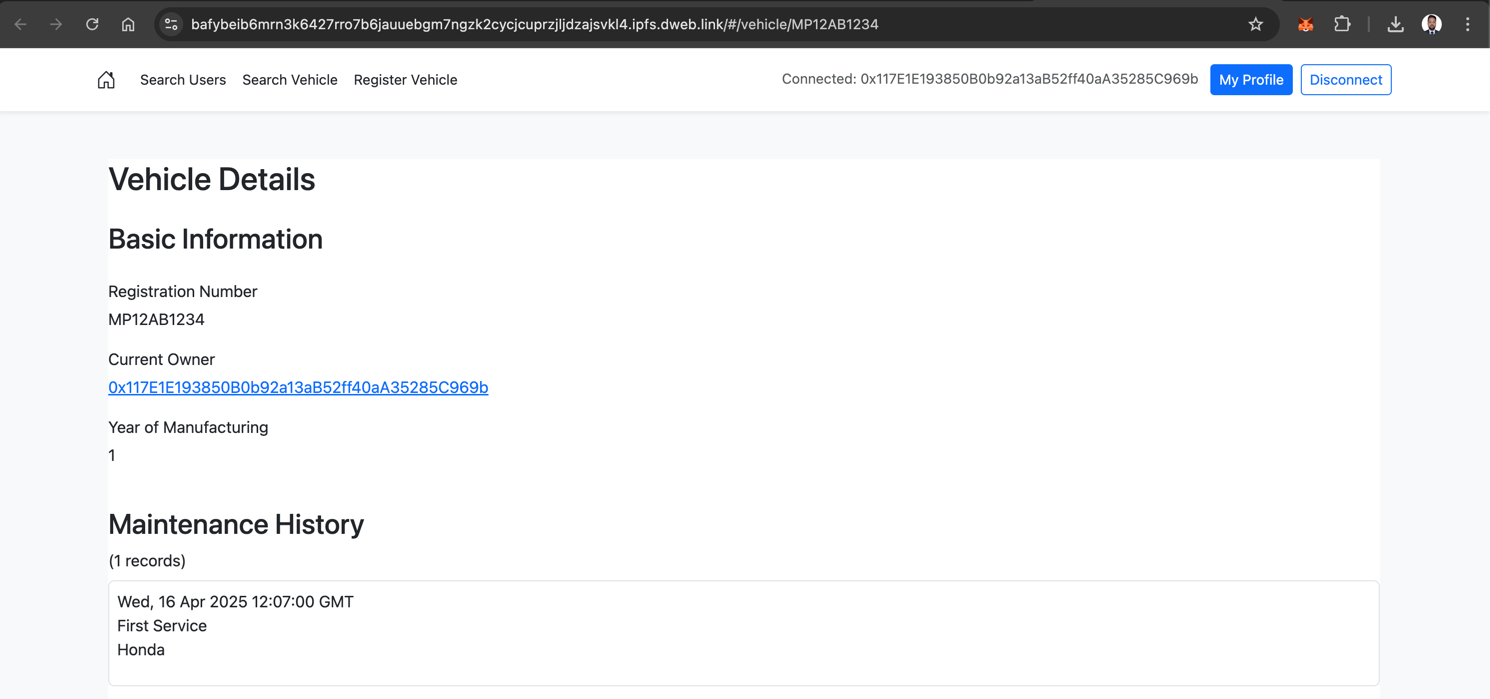
\includegraphics[width=0.45\textwidth]{screenshots/vehicle detaiils - basic and maintenence history.png}}\quad
        \subfloat[Insurance, Accident \& Ownership]{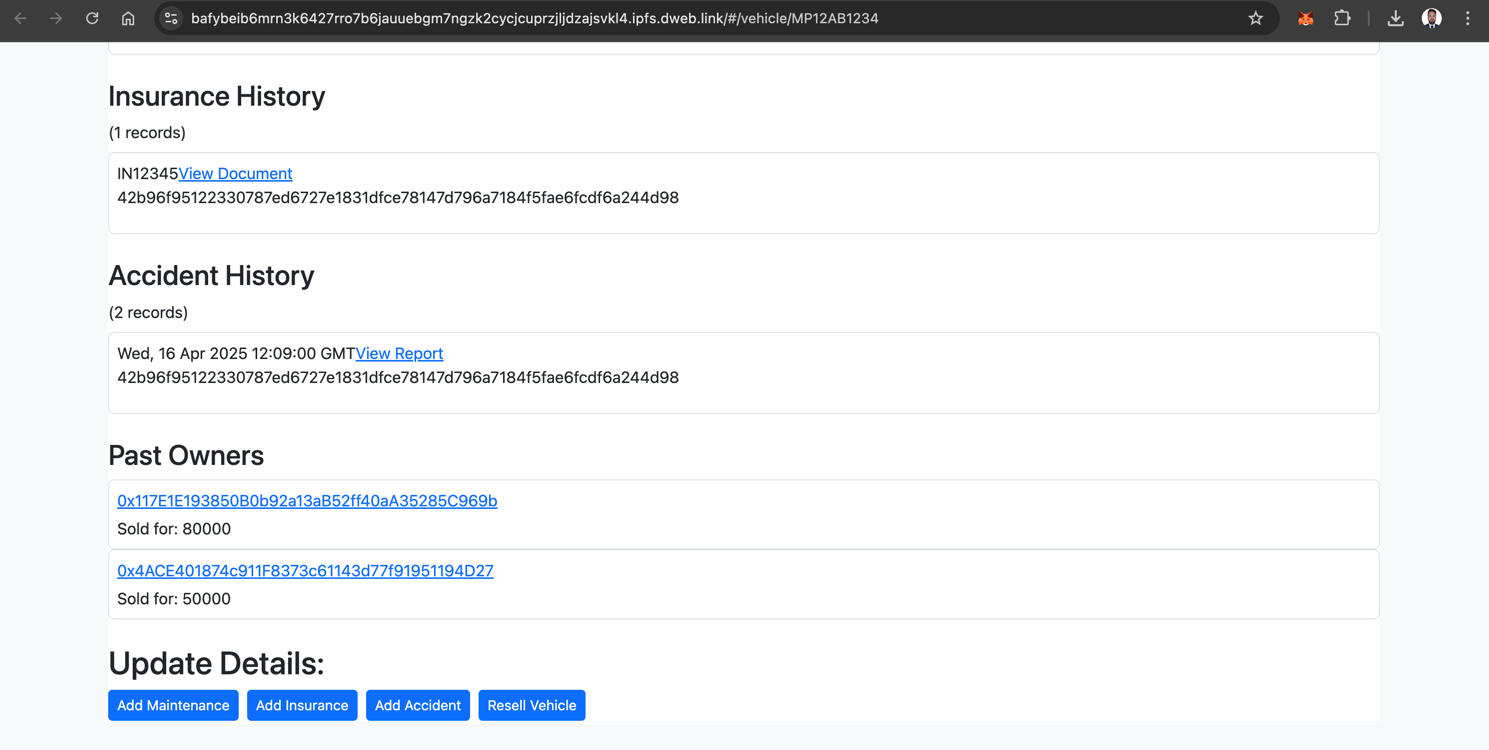
\includegraphics[width=0.45\textwidth]{screenshots/vehicle details - insurance, accident and ownership history.png}}
        \caption{Vehicle Page — Details \& History}
        \label{fig:vehicle-details}
    \end{figure}

    \subsection{Update Maintenance}
    \begin{figure}[H]
        \centering
        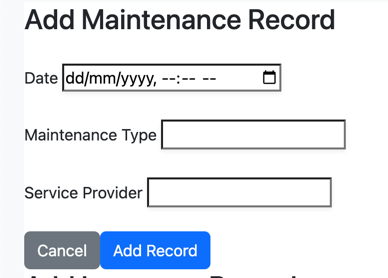
\includegraphics[width=0.6\textwidth]{screenshots/vehicle - add maintenance.png}
        \caption{Add Maintenance Record}
        \label{fig:update-maintenance}
    \end{figure}

    \subsection{Update Accident}
    \begin{figure}[H]
        \centering
        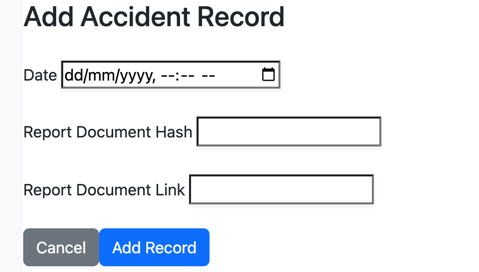
\includegraphics[width=0.6\textwidth]{screenshots/vehicle - add accident record.png}
        \caption{Add Accident Record}
        \label{fig:update-accident}
    \end{figure}

    \subsection{Update Insurance}
    \begin{figure}[H]
        \centering
        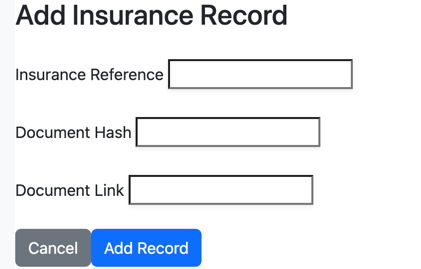
\includegraphics[width=0.6\textwidth]{screenshots/vehicle - add insurance.png}
        \caption{Add Insurance Record}
        \label{fig:update-insurance}
    \end{figure}

    \subsection{Resell Vehicle}
    \begin{figure}[H]
        \centering
        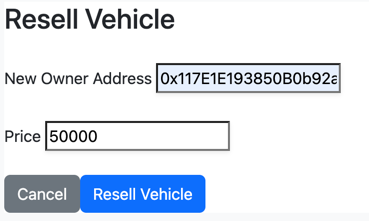
\includegraphics[width=0.6\textwidth]{screenshots/resell vehicle.png}
        \caption{Vehicle Resale Interface}
        \label{fig:resell}
    \end{figure}

    \subsection{Search Vehicle}
    \begin{figure}[H]
        \centering
        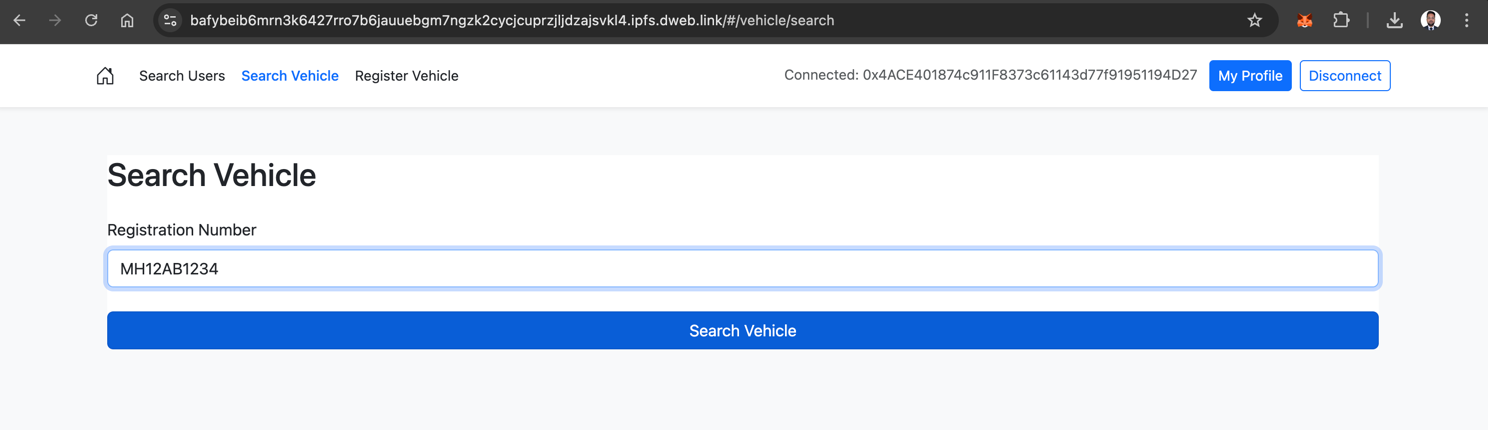
\includegraphics[width=0.6\textwidth]{screenshots/vehicle search.png}
        \caption{Vehicle Search Interface}
        \label{fig:search-vehicle}
    \end{figure}

    \subsection{Search User}
    \begin{figure}[H]
        \centering
        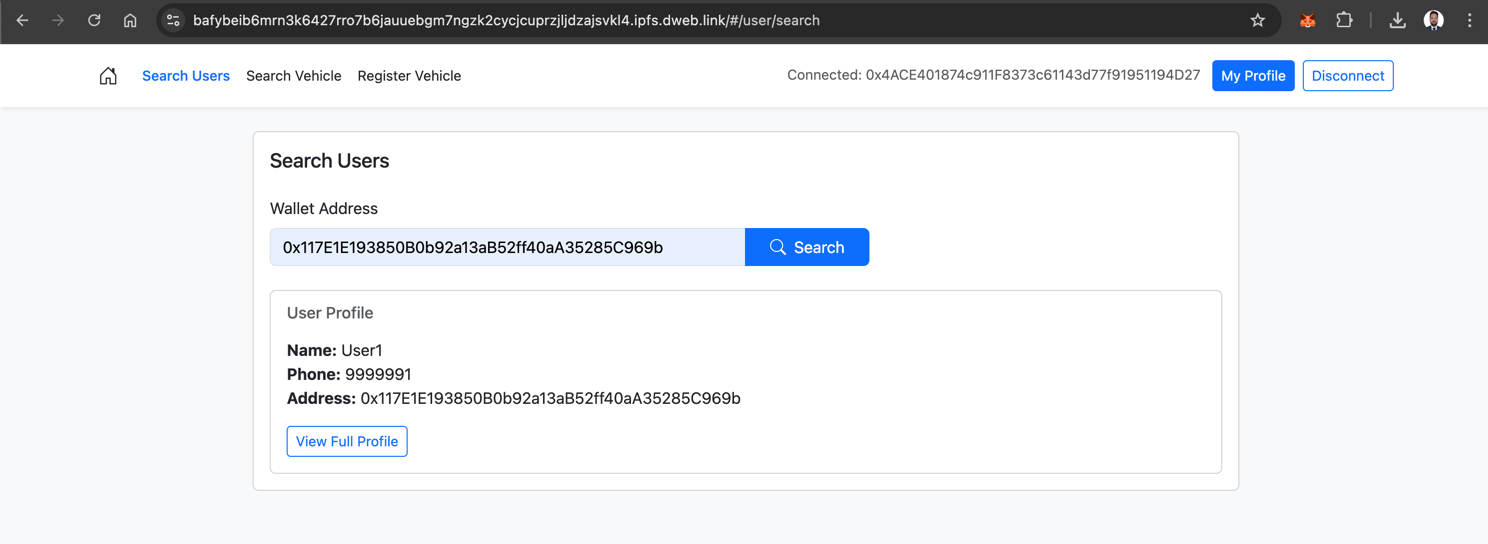
\includegraphics[width=0.6\textwidth]{screenshots/user search.png}
        \caption{User Search Interface}
        \label{fig:search-user}
    \end{figure}

    \subsection{User Profile}
    \begin{figure}[H]
        \centering
        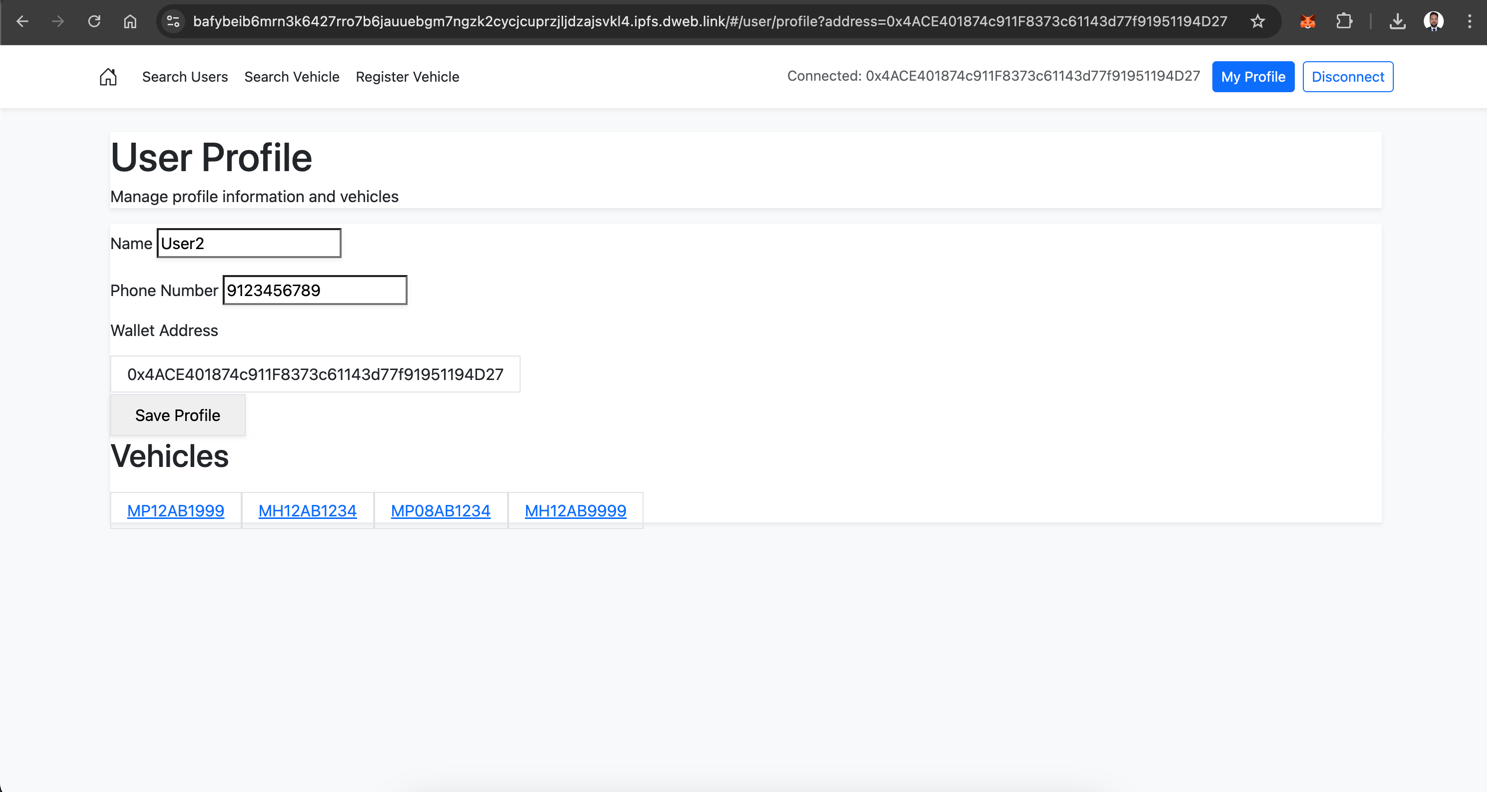
\includegraphics[width=0.6\textwidth]{screenshots/user profile with list of vehicle.png}
        \caption{User Profile Page}
        \label{fig:user-profile}
    \end{figure}

    \subsection{MetaMask Transaction Request}
    \begin{figure}[H]
        \centering
        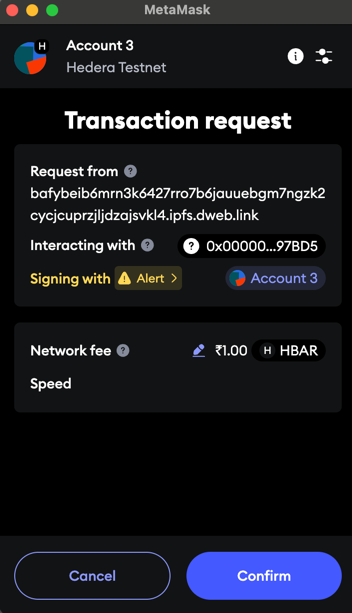
\includegraphics[width=0.6\textwidth]{screenshots/metamask transaction request.png}
        \caption{MetaMask Transaction Request}
        \label{fig:txn-request}
    \end{figure}


    \section{Sample Interactions}

    \subsection{Vehicle Registration}
    \begin{enumerate}
        \item User connects wallet
        \begin{itemize}
            \item Click "Connect Wallet"
            \item Approve MetaMask popup
            \item Verify connection
        \end{itemize}

        \item Fills registration form
        \begin{itemize}
            \item Enter vehicle details
        \end{itemize}

        \item Submits transaction
        \begin{itemize}
            \item Click "Register"
            \item Confirm transaction
            \item Wait for confirmation
        \end{itemize}

        \item Confirms in MetaMask
        \begin{itemize}
            \item Review transaction
            \item Approve gas fee
            \item Sign transaction
        \end{itemize}

        \item Receives confirmation
        \begin{itemize}
            \item View success message
            \item Download certificate
            \item Check transaction status
        \end{itemize}
    \end{enumerate}

    \subsection{Vehicle Search}
    \begin{enumerate}
        \item Enter Registration number

        \item Navigate to vehicle page

        \item Access detailed information
        \begin{itemize}
            \item View vehicle details
            \item Check ownership history
            \item View documents
        \end{itemize}

        \item Verify ownership
        \begin{itemize}
            \item Check current owner
            \item View transfer history
            \item Verify authenticity
        \end{itemize}
    \end{enumerate}


    \section{Security \& Data Integrity}

    \subsection{Security Measures}
    \begin{itemize}
        \item Blockchain-based data storage
        \begin{itemize}
            \item Distributed ledger
            \item Cryptographic hashing
            \item Consensus mechanism
        \end{itemize}

        \item Smart contract access control
        \begin{itemize}
            \item Vehicle: only current owner can update details or resell a vehicle
            \item User: Current user can only update own profile
        \end{itemize}

        \item Wallet authentication
        \begin{itemize}
            \item Private key security
            \item Transaction signing
        \end{itemize}
    \end{itemize}

    \subsection{Data Integrity}
    \begin{itemize}
        \item Immutable records
        \begin{itemize}
            \item Blockchain storage
            \item Hash verification
            \item Timestamp validation
        \end{itemize}

        \item Transparent transactions
        \begin{itemize}
            \item Public ledger
            \item Transaction history
        \end{itemize}
    \end{itemize}


    \section{Deployment}

    \subsection{Deployment}
    The application is deployed on:
    \begin{itemize}
        \item Frontend: IPFS Gateway (please refer to Appendix \ref{app:Deployment})
        \begin{itemize}
            \item Angular production build
            \item Deployment of build files on IPFS using \href{https://app.pinata.cloud/}{Pinata}
        \end{itemize}

        \item Smart Contracts: Hedera Testnet
        \begin{itemize}
            \item Contract compilation and deployment
            \item Address verification
            \item ABI management
        \end{itemize}

        \item Distributed Storage: IPFS
        \begin{itemize}
            \item Document storage
            \item Distributed Applicatoin deployment
        \end{itemize}
    \end{itemize}


    \section{Challenges Faced}
    \begin{itemize}
        \item Integration with Hedera Network
        \begin{itemize}
            \item Transaction handling
            \item Gas optimization
            \item Calling one transaction from other
        \end{itemize}

        \item Wallet connectivity issues
        \begin{itemize}
            \item Account switching
        \end{itemize}

        \item Gas fee optimization
        \begin{itemize}
            \item Contract optimization
        \end{itemize}

        \item User experience in blockchain transactions
        \begin{itemize}
            \item Transaction waiting
            \item Error handling
            \item Status updates
        \end{itemize}

        \item Data storage limitations
        \begin{itemize}
            \item Documents storage
        \end{itemize}
    \end{itemize}


    \section{Future Scope}

    \subsection{Additional Application Features}
    \begin{itemize}
        \item Trusted nodes
        \begin{itemize}
            \item Onboard car manufacturers and government agencies to integrate their data with this system.
        \end{itemize}

        \item Purchasing with cryptocurrency
        \begin{itemize}
            \item Add support for buying and selling using HBAR itself, or any cryptocurrency.
        \end{itemize}

        \item Integration with Web3 Storage
        \begin{itemize}
            \item Integration with IPFS, Pinata etc. for document tracking and uploads.
        \end{itemize}

        \item Servicing history
        \begin{itemize}
            \item Add support for more data points like servicing history, kilometres driven etc.
        \end{itemize}
    \end{itemize}

    \subsection{Enhanced User Features}
    \begin{itemize}
        \item Role-based access control
        \begin{itemize}
            \item Admin privileges
            \item Service provider access
            \item Government access
        \end{itemize}

        \item Multi-signature transactions
        \begin{itemize}
            \item Joint ownership
            \item Corporate accounts
            \item Escrow services
        \end{itemize}

        \item Advanced search capabilities
        \begin{itemize}
            \item Fuzzy search
            \item Filter combinations
            \item Saved searches
        \end{itemize}
    \end{itemize}

    \subsection{System Improvements}
    \begin{itemize}
        \item Performance optimization
        \begin{itemize}
            \item Caching mechanisms
            \item Query optimization
            \item Load balancing
        \end{itemize}

        \item Enhanced security features
        \begin{itemize}
            \item Multi-factor authentication
            \item Biometric verification
            \item Advanced encryption
        \end{itemize}

        \item Mobile responsiveness
        \begin{itemize}
            \item Progressive Web App
            \item Native mobile apps
            \item Offline capabilities
        \end{itemize}
    \end{itemize}

    \subsection{Integration Possibilities}
    \begin{itemize}
        \item Insurance providers
        \begin{itemize}
            \item Policy management
            \item Claim processing
            \item Premium calculation
        \end{itemize}

        \item Service centers
        \begin{itemize}
            \item Appointment scheduling
            \item Service tracking
            \item Parts inventory
        \end{itemize}

        \item Government agencies
        \begin{itemize}
            \item Tax collection
            \item Regulation compliance
            \item Law enforcement
        \end{itemize}
    \end{itemize}


    \section{Conclusion}
    The Vehicle Management System on Hedera Network provides a secure, transparent, and efficient solution for vehicle registration and management. By leveraging blockchain technology, it ensures data integrity and provides a tamper-proof record of vehicle information. The system's modular architecture and comprehensive feature set make it a robust solution for modern vehicle management needs.

    Key achievements include:
    \begin{itemize}
        \item Successful implementation of decentralized vehicle registration using smart contracts
        \item Secure and transparent ownership transfer mechanism
        \item User-friendly interface for system interaction
        \item Robust security measures and data integrity
    \end{itemize}

    The system demonstrates the practical application of blockchain technology in solving real-world problems related to vehicle management and sets a foundation for future enhancements and integrations.


    \section{References}
    \begin{enumerate}
        \item Hedera Documentation
        \begin{itemize}
            \item Smart Contract Service
            \item Consensus Service
            \item Token Service
        \end{itemize}

        \item Solidity Documentation
        \begin{itemize}
            \item Language Specification
            \item Security Considerations
            \item Best Practices
        \end{itemize}

        \item Angular Documentation
        \begin{itemize}
            \item Component Architecture
            \item Service Implementation
            \item Routing System
        \end{itemize}

        \item Web3.js Documentation
        \begin{itemize}
            \item Contract Interaction
            \item Event Handling
            \item Transaction Management
        \end{itemize}

        \item MetaMask Documentation
        \begin{itemize}
            \item Wallet Integration
            \item Transaction Signing
            \item Network Management
        \end{itemize}
    \end{enumerate}


    \section{Appendix}

    \subsection{Smart Contract Code}
    \label{app:contracts}

    \subsubsection{VehicleLedger.sol}
    \begin{minted}{solidity}
// SPDX-License-Identifier: MIT
pragma solidity ^0.8.0;

contract VehicleLedger {
    struct Maintenance {
        uint date;
        string maintenanceType;
        string serviceProvider;
    }

    struct Insurance {
        string insuranceRef;
        string docHash;
        string docLink;
    }

    struct Accident {
        uint date;
        string reportDocHash;
        string reportDocLink;
    }

    struct Vehicle {
        string regNo;
        address currentOwner;
        address[] pastOwners;
        uint yearOfManufacturing;
        Maintenance[] maintenanceHistory;
        Insurance[] insuranceHistory;
        Accident[] accidentHistory;
        uint[] resellAmounts;
    }

    mapping(string => Vehicle) public vehicles;
    address public userProfileAddress; // Address of the UserProfile contract

    address public owner;

    constructor() {
        owner = msg.sender;
    }

    modifier onlyOwner() {
        require(msg.sender == owner, "Only the creator can call this function");
        _;
    }

    // Set the UserProfile contract address via a method.
    function setUserProfileAddress(address _addr) public onlyOwner {
        userProfileAddress = _addr;
    }

    // Register a new vehicle.
    // Registration accepts only the registration number and year. History entries can be appended later.
    function registerVehicle(string calldata regNo, uint yearOfManufacturing) external {
        // Ensure vehicle doesn't already exist.
        require(vehicles[regNo].yearOfManufacturing == 0, "Vehicle already registered");

        Vehicle storage vehicle = vehicles[regNo];
        vehicle.regNo = regNo;
        vehicle.currentOwner = msg.sender;
        vehicle.yearOfManufacturing = yearOfManufacturing;

        // Call UserProfile to add this vehicle to the user's profile.
        if (userProfileAddress != address(0)) {
            (bool success,) = userProfileAddress.call(
                abi.encodeWithSignature("addVehicle(address,string)", msg.sender, regNo)
            );
            require(success, "addVehicle call failed");
        }
    }

    // Append a maintenance entry. Only the current owner can update.
    function addMaintenance(string calldata regNo, uint date, string calldata maintenanceType, string calldata serviceProvider) external {
        Vehicle storage vehicle = vehicles[regNo];
        require(vehicle.currentOwner != address(0), "Vehicle not found");
        require(vehicle.currentOwner == msg.sender, "Caller is not the owner");
        vehicle.maintenanceHistory.push(Maintenance(date, maintenanceType, serviceProvider));
    }

    // Append an insurance entry. Only the current owner can update.
    function addInsurance(string calldata regNo, string calldata insuranceRef, string calldata docHash, string calldata docLink) external {
        Vehicle storage vehicle = vehicles[regNo];
        require(vehicle.currentOwner != address(0), "Vehicle not found");
        require(vehicle.currentOwner == msg.sender, "Caller is not the owner");
        vehicle.insuranceHistory.push(Insurance(insuranceRef, docHash, docLink));
    }

    // Append an accident entry. Only the current owner can update.
    function addAccident(string calldata regNo, uint date, string calldata reportDocHash, string calldata reportDocLink) external {
        Vehicle storage vehicle = vehicles[regNo];
        require(vehicle.currentOwner != address(0), "Vehicle not found");
        require(vehicle.currentOwner == msg.sender, "Caller is not the owner");
        vehicle.accidentHistory.push(Accident(date, reportDocHash, reportDocLink));
    }

    // Resale a vehicle.
    // Only the current owner can sell. Records resale amount history.
    function resaleVehicle(string calldata regNo, address newOwner, uint resellAmount) external {
        Vehicle storage vehicle = vehicles[regNo];
        require(vehicle.currentOwner == msg.sender, "Caller is not the owner");

        // Record current owner in past owners.
        vehicle.pastOwners.push(msg.sender);
        vehicle.currentOwner = newOwner;
        vehicle.resellAmounts.push(resellAmount);

        // Update UserProfile: remove vehicle from seller and add to buyer.
        if (userProfileAddress != address(0)) {
            (bool success,) = userProfileAddress.call(
                abi.encodeWithSignature("removeVehicle(address,string)", msg.sender, regNo)
            );
            require(success, "removeVehicle call failed");

            (bool successAdd,) = userProfileAddress.call(
                abi.encodeWithSignature("addVehicle(address,string)", newOwner, regNo)
            );
            require(successAdd, "addVehicle call failed");
        }
    }

    function getVehicleDetails(string calldata regNo) external view returns (
        string memory,
        address,
        address[] memory,
        uint,
        uint,
        uint,
        uint,
        uint
    ) {
        Vehicle storage vehicle = vehicles[regNo];
        require(vehicle.yearOfManufacturing != 0, "Vehicle not found");
        return (
            vehicle.regNo,
            vehicle.currentOwner,
            vehicle.pastOwners,
            vehicle.yearOfManufacturing,
            vehicle.maintenanceHistory.length,
            vehicle.insuranceHistory.length,
            vehicle.accidentHistory.length,
            vehicle.resellAmounts.length
        );
    }

    function getMaintenanceHistory(string calldata regNo) external view returns (Maintenance[] memory) {
        return vehicles[regNo].maintenanceHistory;
    }

    function getInsuranceHistory(string calldata regNo) external view returns (Insurance[] memory) {
        return vehicles[regNo].insuranceHistory;
    }

    function getAccidentHistory(string calldata regNo) external view returns (Accident[] memory) {
        return vehicles[regNo].accidentHistory;
    }

    function getResellHistory(string calldata regNo) external view returns (uint[] memory) {
        return vehicles[regNo].resellAmounts;
    }

    function getPastOwnerHistory(string calldata regNo) external view returns (address[] memory) {
        return vehicles[regNo].pastOwners;
    }
}
    \end{minted}

    \subsubsection{UserProfile.sol}
    \begin{minted}{solidity}
// SPDX-License-Identifier: MIT
pragma solidity ^0.8.0;

contract UserProfile {
    struct User {
        address walletAddress;
        string name;
        string phone;
        string[] vehicles; // vehicle registration numbers owned by user
    }

    mapping(address => User) public users;

    // Internal function to add a user with no details if not present.
    function ensureUserExists(address userAddr) internal {
        if (users[userAddr].walletAddress == address(0)) {
            // Create a new user with default empty details.
            users[userAddr] = User({
                walletAddress: userAddr,
                name: "",
                phone: "",
                vehicles: new string[](0)
            });
        }
    }

    // Create or update user profile.
    // Called by the user themselves.
    function updateUserProfile(string calldata _name, string calldata _phone) external {
        ensureUserExists(msg.sender);
        User storage user = users[msg.sender];
        user.name = _name;
        user.phone = _phone;
    }

    // Append a vehicle registration number to user's profile.
    // Called from from the VehicleLedger contract.
    function addVehicle(address userAddr, string calldata regNo) external {
        ensureUserExists(userAddr);
        users[userAddr].vehicles.push(regNo);
    }

    // Remove a vehicle registration number from user's profile.
    // Called from the VehicleLedger contract.
    function removeVehicle(address userAddr, string calldata regNo) external {
        User storage user = users[userAddr];
        uint len = user.vehicles.length;
        for (uint i = 0; i < len; i++) {
            if (keccak256(bytes(user.vehicles[i])) == keccak256(bytes(regNo))) {
                // Remove element by swapping with last and popping the array.
                user.vehicles[i] = user.vehicles[len - 1];
                user.vehicles.pop();
                break;
            }
        }
    }

    // Retrieve user profile details.
    // Note: This functions is not marked as view, because they may modify state by ensuring the user exists.
    function getUserProfile(address userAddr) external returns (string memory, string memory, string[] memory) {
        ensureUserExists(userAddr);
        User storage user = users[userAddr];
        return (user.name, user.phone, user.vehicles);
    }

    // Getter for the wallet address associated with the user profile.
    // Note: This functions is not marked as view, because they may modify state by ensuring the user exists.
    function getUserWallet(address userAddr) external returns (address) {
        ensureUserExists(userAddr);
        return users[userAddr].walletAddress;
    }

    // Getter for the user's name.
    function getUserName(address userAddr) external view returns (string memory) {
        return users[userAddr].name;
    }

    // Getter for the user's phone number.
    function getUserPhone(address userAddr) external view returns (string memory) {
        return users[userAddr].phone;
    }

    // Getter for the array of vehicle registration numbers.
    function getUserVehicles(address userAddr) external view returns (string[] memory) {
        return users[userAddr].vehicles;
    }
}
    \end{minted}

    \subsection{Deployment Guide}
    \begin{enumerate}
        \item Prerequisites
        \begin{itemize}
            \item Node.js 20.11.0 or later
            \item Angular CLI 19.2.0
            \item MetaMask wallet
            \item Hedera testnet account
        \end{itemize}

        \item Setup Steps
        \begin{itemize}
            \item Clone repository
            \item Install dependencies
            \item Configure environment variables
            \item Deploy smart contracts
            \item Start frontend application
        \end{itemize}

        \item Testing
        \begin{itemize}
            \item Run unit tests
            \item Execute integration tests
            \item Perform security audits
        \end{itemize}
    \end{enumerate}


    \section{Deployment Information}
    The application is deployed with the following details:

    \subsection{Project Repository}
    \begin{itemize}
        \item GitHub: \url{https://github.com/dharmendra912/VehicleResellingDapp}
    \end{itemize}

    \subsection{Smart Contracts}
    \begin{itemize}
        \item VehicleLedger.sol
        \begin{itemize}
            \item Contract ID: 0.0.5864405
            \item EVM Address: 0x0000000000000000000000000000000000597bd5
            \item Explorer: \href{https://hashscan.io/testnet/contract/0.0.5864405}{Contract Explorer}
        \end{itemize}

        \item UserProfile.sol
        \begin{itemize}
            \item Contract ID: 0.0.5864437
            \item EVM Address: 0x0000000000000000000000000000000000597bf5
            \item Explorer: \href{https://hashscan.io/testnet/contract/0.0.5864437}{Contract Explorer}
        \end{itemize}
    \end{itemize}

    \label{app:Deployment}

    \subsection{IPFS Gateway}
    The frontend is deployed on IPFS with the following gateway:
    \begin{itemize}
        \item \href{https://w3s.link/ipfs/bafybeib6mrn3k6427rro7b6jauuebgm7ngzk2cycjcuprzjljdzajsvkl4/}{IPFS Gateway}
    \end{itemize}

\end{document}
